%! Author = alexis
%! Date = 14/06/2022

% Document






%Typically, social network visualization and visual analytics is used at the end of this tedious process for analysis goals, but it is not uncommon to find errors and inconsistencies, or to realize the network do not match the analysis goals.
%\va could therefore be useful as a method to improve the overall workflow of historians, to find errors and inconsistencies before the final analysis steps, with the help of exploration.
%It is also not yet completely clear what types of representations and interactions are efficients for social historians to answer their diverstiy of questions and problematics.
%They usually rely on famous softwares such as Gephi and Pajek to visualize their networks with node-link diagrams and compute structural network measures, but more complex visualizations and interactions are needed to represent other network models are satisfy historians needs.





\chapter{Introduction}



Historical Social Network Analysis is a method---sometimes referred as a paradigm---followed by social historians to study sociological phenomena through the observation of relationships of actors of the past, modeled into a network.
%The usage of networks as an abstraction to represent and study social relationships---such as friendships, kinship, or business ties---grew in popularity in the last 40 years \cite{freemanDevelopmentSocialNetwork2004, tabassumSocialNetworkAnalysis2018}, especially in our time when many of our digital connections and interactions take explicit network shapes\footnote{This analogy goes to the point that the term ``Social Network'' can refer both to the scientific sociological concept of the modeling of social relationships and the social media platforms such as Facebook.}.
The usage of networks as an abstraction to represent and study social relationships---such as friendships, kinship, or business ties---grew in popularity in the last 40 years \cite{freemanDevelopmentSocialNetwork2004, tabassumSocialNetworkAnalysis2018} and is a powerful metaphor especially in our time when many of our digital connections and interactions take explicit network structure\footnote{This analogy goes to the point that the term ``Social Network'' can refer both to the sociological metaphor for social relationship and the social media platforms such as Facebook.}.
Historians leverage historical documents---which are at the core of their profession\cite{langloisIntroductionAuxEtudes2014}---to extract relationships between actors of interest that they model with networks constructed from nodes and links that respectively represent actors (often persons) and relationships.
Using social network visualization techniques and leveraging network measures and computations, they can then test hypotheses they have and gain insight on the structural aspect of the relational phenomena they are studying\cite{wetherellHistoricalSocialNetwork1998, kerschbaumerPowerNetworksProspects2015}.
%They typically use Social Network Visualization and Analysis tools such as Gephi \cite{Gephi} to test hypotheses they have, and gain insight on the structure of relationships they are studying.
This approach has been followed successfully to study various subjects such as kinship \cite{hambergerKinshipNetworkAnalysis2011}, entrepreneurship \cite{rubio-mondejarWomenEntrepreneursFamily2022}, maritime routes \cite{larsonThomasTartaronMaritime2014}, political power \cite{padgettRobustActionRise1993} and oppositions \cite{osaSolidarityContentionNetworks2003}, and persecution \cite{merckléPeutonModéliserPersécution2018}.
Yet, history is considered by many as a literary and qualitative science, and many critics emerged concerning quantitative and network methods \cite{lepetitHistoireQuantitativeDeux1989, karila-cohenNouvellesCuisinesHistoire2018, lemercier12FormalNetwork2015}, such as the leading to trivial conclusions, anachronisms, and mismatches between network and historical concepts.
Moreover, quantitative and network analysis are complex processes, and demand many efforts in data collection, cleaning and processing before being able to make efficient observations.

Social historians have to take many annotation and modeling decisions, concerning \emph{what} to model from their sources into a network, and \emph{how} to model it \cite{cristofoliAuxSourcesGrands2008, dufournaudRechercheEmpiriqueHistoire2015}, \ie should the information of interest be represented as a node, a link, an attribute, or not reflected in the network at all.
Practically, they usually use adhoc processing and analysis scripts to transform historical documents to analyzable networks, which is time-consuming, sometimes to end up with trivial or hard to interpret results \cite{alkadi2022}.
Still, HSNA led to many highly regarded studies with thorough conclusions, such as the study of families of power in Florence by Padgett and Ansell where they explained the rise of the Medici family through their central position in the economical, political, and trading networks of powerful families \cite{padgettRobustActionRise1993}.

The usage of visuals to graphically display networks is common in \sna as it allows to unfold the structure of networks to the eyes, thus letting social scientists confirm hypotheses they had when collecting and exploring their data aswell as gaining new insight through the discovery of interesting patterns and trends \cite{cristofoliPrincipesUsagesDessins}.
Images of networks also constitute an efficient mean of communication, especially in scientific productions \cite{freemanVisualizingSocialNetworks2000}.
Many visualization techniques and softwares have thus been developed since the birth of \sna, but most popular tools are usually not designed for historians specifically and usually enforce traditional network models without proposing exploration mechanisms, beyond allowing to look at the network structure and computed measures.
In this thesis, we therefore investigate how visualization can support social historians in their overall process, starting at the acquisition of their document, and also at the analysis step, \ie  how visualization interfaces can support social historians in answering their questions with the right level of expressiveness, usability, and traceability.



%In parallel, the data mining community proposed many algorithms in the last decades to automatically find interesting patterns and analyzing social networks through tasks such as clustering, node classification, or embedding.
%Social Network Visualization interfaces started to incorporate those techniques allowing social scientists to leverage those algorithms to gain insight on their data directly in their analysis workflow.



%Social Network Visualization is typically used as a way to unfold the hidden structure of relationships to the eyes, and communicate findings in scientific productions.
%However, most used \snv softwares usually enforce traditional network models and do not propose exploration mechanisms.
%The goal of this thesis is therefore to explore how \va can assist social historians in their \hsna process,
%first on the data cleaning, acquisition, and modeling steps, and secondly from an analytical standpoint, for historians to be able to answer their historical questions with the right level of expressiveness, usability, and traceability.


%Social scientists such as historians and sociologists want to make sense of the structure and evolutions of the social relationships between people of a given place and time.
%Social Network Analysis (SNA), also called Historical Social Network Analysis (HSNA) when applied to historical data, is one of the main methods ---sometimes referred to as a paradigm---to achieve this goal, and grew in popularity in recent years as the concept of networks became a widespread abstraction in many empirical sciences.
%It consists in modeling the social relationships between agents---such as persons and organizations---as a network and studying its local and global structure to make sociological conclusions, based on real observations.
%Compared to other more classical sociological approaches, ``it is based on an assumption of the importance of relationships among interacting units.
%The social network perspective encompasses theories, models, and applications that are expressed in terms of relational concepts or processes.''\cite{wassermanSocialNetworkAnalysis1994}.
%Social historians rely on textual documents---such as marriage acts, birth certificate, and migration acts---and try to exhaustively extract all mentions of social relationships between persons that they model into a social network, where the nodes usually model persons, and links social relationships.
%Using mathematical computations and measures to characterize the network's structure, they are able to make sociological conclusions on relational sociological phenomena based on real observations.
%%Usually, agents are represented as nodes in the network, while the links model social relationships, such as friendships, business, or family links.
%%To construct such networks, social historians rely on textual documents---such as marriage acts, birth certificate, and migration acts---and try to exhaustively extract all mentions of persons and their social relationships that they then model into a social network.
%%Social Historians can afterwards apply social network methods based on mathematical computations and measures to characterize the network's structure to finally make sociological conclusions.
%
%%To construct such networks, social scientists try to exhaustively list all the persons in a restricted time and place with all their social ties and create a network from it.
%%The resulting network is considered to be a good model of the social reality, thus allowing to study the structure and dynamics of the social fabric of a period, by studying the network in itself.
%They also rely on Social Network Visualization to make useful representations of social networks and are starting to use Visual Analytics (VA) tools that allow them an effective exploration and analysis of this type of data, based on direct interaction and manipulation to find relevant patterns and trends.
%%In parallel, a lot of work has been done in network visualization and specifically Social Network Visualization (SNV) to make useful representations of social networks, and visual analytics tools allowing an effective exploration and analysis of this type of data.
%However, the process leading to the analyzable network from the historical documents is quite complex and not well documented.
%Specifically, historians can model their networks in many ways, and choosing a model loosely can lead to simplifications and distortions in the social reality and the final analyses.
%Annotating the documents and cleaning the extracted information is also not trivial and can lead to errors and biases.
%Most VA tools currently focus on the analysis part only of the process and do not help social historians in their annotation, cleaning, and modeling steps.
%Moreover, automatic algorithms capabilities such as clustering are often available in SNA tools to help users make sense of the network structure, but interpreting the results from a sociological perspective is complicated especially without guidance, and social scientists have become frustrated by the use of such software\cite{lemercierBackSourcesPracticing2021}.
%%The goal of this thesis is therefore to see how VA can be useful to social historians, in their entire process.
%%Particularly, we first characterize the HSNA process and from this,
%The goals of this thesis are therefore first to characterize the HSNA process of social historians, and from characterizing recurring pitfalls, see how VA can help them in this complex process.
%Particularly, we study how VA can help them follow complex analyses to answer their sociological questions while keeping a high level of simplicity, traceability, usability, and with the right level of control.
%
%
%%This thesis's goal is to 1) shed light on the workflow of historians following a network analysis, to provide research directions towards new VA interface to help social scientists in their overall work, 2) provide VA interfaces which focus on complex interactions to help social scientists answer their complex questions while 3) focusing on the usability of those systems, especially concerning the traceability and interpretations of the results.



\section{Social History and Historical Social Network Analysis}

HSNA is now a widely used method among historians to study relational phenomena like kinship, business, and institutions of the past, using network concepts and methods.
%It appeared as an effective method to study their sources after a long process of methodological shifts and discussions\cite{cristofoliAuxSourcesGrands2008}.
%It is though a relatively new approach in History, where methodology changed through the years.
%History is the science of retrieving and characterizing facts about the past, in all their complexity.
We can trace it back to the birth of Social History with the ``Annales School'' in the 1930s, where Historians gained interest in socio-economic questions and started to rely heavily on the exhaustive extraction and analysis of historical documents coming from archives\cite{blochApologiePourHistoire1949, prost2014}.
Beforehand, History was mainly political and event-centered, as the majority of work consisted in narrating and characterizing specific events---such as wars and diplomatic alliances---while eliciting their causes and consequences, and describing the lives of historic figures, such as sovereigns \cite{prost2014}.
Social History shifted the focus by aiming to link together sociological, economical, and political issues and by placing individuals at the center of these questions\cite{tilly1984retrieving}.
Later on in the 1960s, with the development of Computer Science, historians started to use quantitative methods to analyze data extracted from historical documents and make conclusions grounded in statistical results, in various subjects such as demographics\cite{henryRegistresParoissiauxHistoire1956} and economics\cite{goldinCliometricsNobel1995}.
Around the same time, the use and study of networks started to become popular in various disciplines to study real-world relational phenomena based on mathematical computations and measures, especially in sociology and anthropology.
A network is an abstraction based on graph theory concepts which can be used to model phenomena based on relationships (called links) between entities (called nodes).

%More recently, with the development of network science and computer science, sociologists started to study social phenomena and relationships from a network perspective.
%A network is an abstraction based on graph theory concepts used to model phenomena based on relationships between entities, made of nodes and links.
Sociologists appropriated this concept to model social relationships between agents of interest, allowing them to study the sociological structure of groups of interest---such as families, institutions, and companies---and concepts like friendship, oppression, and diffusion using real world observation and mathematical computations.
This SNA approach allows to ground results in formal network measures and metrics based on real observations instead of relying on traditional social categories such as age, job, and gender\cite{freemanDevelopmentSocialNetwork2004}.
This shift in the object of study from traditional social classes and aggregates to the observation of relationships of individuals remind the microhistoria movement \cite{ginzburgMicrohistoire1981} which theorized that following the life of single individuals and groups allows to make higher level conclusions about the structures they live in.
Social historians followed this tradition and started to appropriate network concepts to study relational aspects of the past and formalized it under the term Historical Network Research or Historical Social Network Analysis (HSNA)\cite{wetherellHistoricalSocialNetwork1998}.
However, historians do not have the possibility to run surveys or directly observe interactions of the past and are thus constrained by the information contained in historical documents they find in archives.
These documents can be anything mentioning social relationships between actors of interest, such as marriage acts, birth certificates, census, migration acts, business transactions, journals.
After selecting a corpus of documents, they typically read and inspect in depth several documents while taking notes to have a deeper insight on the content of the sources, which allow them to start eliciting hypotheses.
Following this exploration phase, they manually annotate each document and encode the desired information---the mention of persons and their social relationship in the case of a future network analysis.
%they manually annotate each document to extract the mentions of persons along their relationships to model those with a network.
%After selecting a corpus of documents, they manually annotate each document to extract the mentions of persons along their relationships to model those with a network.
This is a long and tedious process that can result in small to large networks that they analyze using network measures to make conclusions on the structure of social groups or social behaviour of individual of interests.

The investigation and reading of the historical documents is therefore an exploratory process, where historians start to generate sociological hypotheses from the continuous extraction of insight and revelations of this process, similarly to the grounded theory \cite{glaserDiscoveryGroundedTheory2010}.
Once they finalised a network, they can test their hypotheses using qualitative or quantitative methods based on quantitative and network measures.
Lemercier and Zalc write ``Although history is not an exact science, counting, comparing, classifying, and modeling are nevertheless useful methods for measuring our degree of doubt or certainty, making our hypotheses explicit, and evaluating the influence of a phenomenon.''\cite{lemercierQuantitativeMethodsHumanities2019}
Social historians, therefore, have hypotheses about their subject of study, that they can back up or refute with the help of quantitative and network results, similarly to the competing hypotheses workflow of Intelligence Analysis\cite{dhamiAnalysisCompetingHypotheses2019}.
By pointing to evidence supporting or refuting hypotheses, they can give insight into the level of the plausibility of different claims.
%To verify their findings, historians rely on Social Network Visualization to represent visually their data.
%It lets them find patterns to confirm or deny hypotheses and communicate their finding.



%Sociologists started to use this concept to model social ties between agents of interest---very often persons---and study social phenomena through the description of the network structure, using the SNA methodology\cite{wassermanSocialNetworkAnalysis1994}.
%It allowed them to leverage quantitative measures from the network to make sociological conclusions based on real observations, instead of relying on traditional social categories such as age, job, and gender\cite{freemanDevelopmentSocialNetwork2004}.
%It has been applied to study various subjects like families, political institutions, schools, friendships, work environments, and sports clubs, with promising results.
%It allowed historians to study relational phenomena of the past---such as families and institutions ---through real social relationships directly extracted from historical documents and modeled into a network.


%Typically, social historians using quantitative and network methods work in a descriptive framework and leverage values and measures to make conclusions.
%%Several subjects are also not well suited for such methods, like microhistoria, narratives, ethnography, or biography.
%Lemercier and Zalc write ``Although history is not an exact science, counting, comparing, classifying, and modeling are nevertheless useful methods for measuring our degree of doubt or certainty, making our hypotheses explicit, and evaluating the influence of a phenomenon.''\cite{lemercierQuantitativeMethodsHumanities2019}
%Social historians, therefore, have hypotheses about their subject of study, that they can back up or refute with the help of quantitative and network results, similarly to the competing hypotheses workflow of Intelligence Analysis\cite{dhamiAnalysisCompetingHypotheses2019}.
%By pointing to evidence supporting or refuting hypotheses, they can give insight into the level of the plausibility of different claims.
%To verify their findings, historians rely on Social Network Visualization to represent visually their data.
%It lets them find patterns to confirm or deny hypotheses and communicate their finding.


%Similarly to sociologists, historians can build a network modeling the social relationships between actors of the past, restricted in a specific period and area they are studying.
%If sociologists can use surveys, experiments, or nowadays, the internet to extract social relationships and construct a social network, historians are restricted by the textual sources they can find.
%Their main source of work to extract social relationships in a rigorous way are historical documents which correspond to traces of specific events linking people together.
%These documents can be marriage acts, birth certificates, census for family and close personal relationships, or migration acts and working contracts for other types of social ties.
%After having a selected corpus, they manually annotate each document to extract the persons mentioned in it along the relationships between them, to finally construct a network from this data.
%This is a long and tedious process which can result in small to large networks that they analyze using mathematical measures to make conclusions on historical phenomena.
%want to analyze to make conclusions on the social dynamics of a population of interest.
%For this complicated task, historians follow what is called a Social Network Analysis (SNA), or more precisely a HIstorical Social Network Analysis (HSNA) which consists in characterizing the structure of the network with measures such as the centrality or the density of some parts of the network to then make conclusions on how people were interacting in the period of interest.


%To help their analysis, and generate new hypotheses, they usually rely on Visual Analytics tools to represent and explore their network. The elaboration of visual tools to represent and explore social networks is called Social Network Visualization.
%Sociologists and historians started to use static representation of networks, using node-links diagrams to have a visual understanding of their data, and to report their findings in publications. With the development of visualization, more complex representations and visual analytics tools emerged, which allow more complex representation and exploration capabilities, with the help of interactions and navigations features. Social networks visual systems such as Gephi or Pajek are now widely used in HNR and SNA by social scientists. Representing their network data and being able to interact with it allows them to rapidly have an overview of it, confirm hypotheses they have and arrange new ones by exploring the network.


\section{Visualization and Visual Analytics}

Visualization is the process of displaying data visually to leverage the human visual system and enhance cognition to gain insight into the data\cite{cardReadingsInformationVisualization1999}.
Using visual abstractions (such as size, color, and position) to display abstract data allows us to rapidly see structure and patterns otherwise hidden in raw text and numbers.
As data keeps growing in size with time due to the increase of hardware and storage capabilities, visualization is a powerful tool to gain insight into the underlying structure of various complex datasets.

Visualization has traditionally been used for confirmatory and communication purposes, particularly in empirical sciences.
By showing data visually, analysts are able to confirm or deny hypotheses and communicate their findings in scientific productions.

%Social scientists following a network analysis typically use node-link diagrams, which allow them to represent a network with circles and lines to respectively represent nodes and links.
%It lets them confirm or deny some of their hypotheses by observing the network structure and communicating their results.

%Visualization is mainly used for confirmatory and communication purposes, particularly in social sciences.
%Analysts generally have hypotheses that they want to test: they collect data, model it, compute measures, and plot the data visually to verify that it matches the results.
%They typically use similar plots to communicate findings, for example in scientific reports and presentations.
However, visualization can also be used for exploration, which can help to understand the underlying structure of data and generate new hypotheses.
Tukey defined this process as Exploratory Data Analysis in the 1960s\cite{tukeyExploratoryDataAnalysis1977}, as a procedure to gain insight into the structure of the data by identifying outliers, trends, and patterns with the usage of visualization and statistical measures.
Social network visualization is used for communication of findings in the field, but is also often following this exploration process as showing the network visually allows social scientists to reveal the structure of their data.
As freeman write ``Images of social networks have provided investigators with new insights about network structures and have helped them to communicate those insights to others''\cite{freemanVisualizingSocialNetworks2000}.
Social scientists very often represent their data using node-link diagrams, that we find in every production of reference in the field \cite{wassermanSocialNetworkAnalysis1994, tabassumSocialNetworkAnalysis2018, sna, lazegaReseaux}.

\begin{figure}[!ht]
    \centering % avoid the use of \begin{center}...\end{center} and use \centering instead (more compact)
    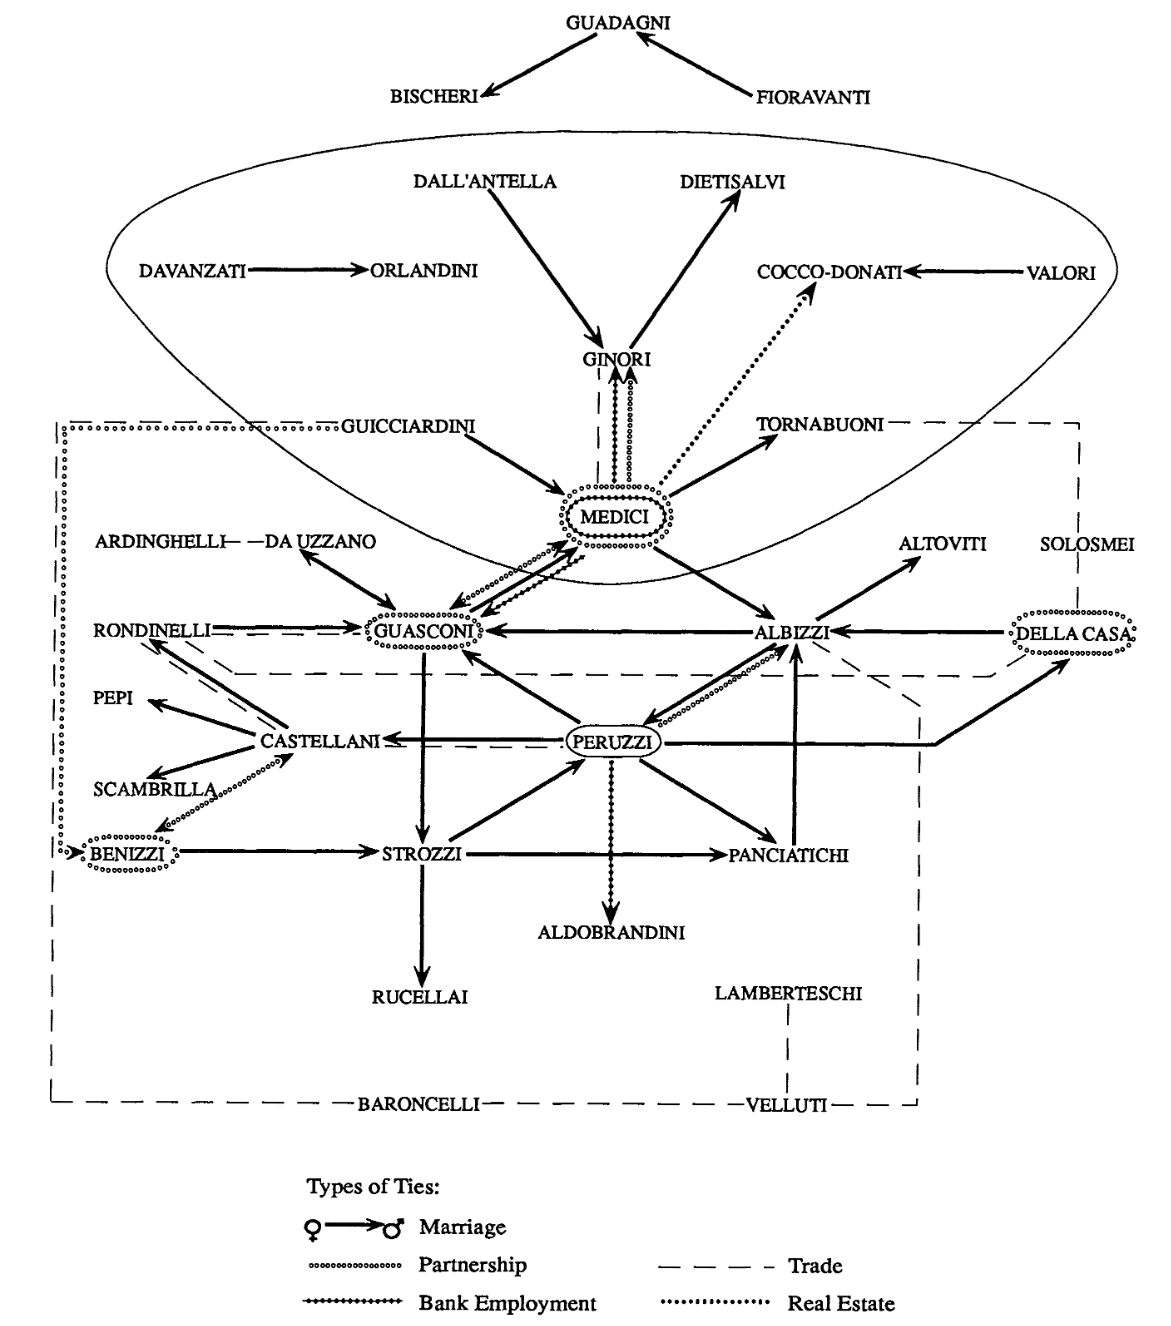
\includegraphics[width=0.8\textwidth]{static/figures/RelatedWork/padgett-Medicis.png}
    \caption{Marriage, partnership. trading, banking, and real estate networks of the powerful families of Florence from \cite{padgettRobustActionRise1993}. We can see the central position in the network of the Medici Family.}
    \label{fig:padgett-medicis}
\end{figure}

\autoref{fig:padgett-medicis} shows a node-link representation of the network constructed by Padgett and Ancell in their work on the Medici.
At that time, diagrams were often drawed by hand, practice which have now been replaced by automatic layout algorithms.

Most visual software for \sna such as Gephi, Pajek, NodeXl, or Ucinet are based on this representation, and allow an exploration of the data with the help of interaction mechanisms and the computation of network measures.

%Interaction in visualization helps this process by letting users navigate more easily on multivariate datasets with the help of direct manipulation of the data.

The detection of patterns and trends can also be facilitated with automatic methods coming from data mining and machine learning fields, directly implemented in the visual analysis loop.
This coupling of visual exploration and automatic data mining algorithms has been coined as Visual Analytics (VA) and is defined as the process of using interactive visualizations, transformations, and models of the data in an interactive analysis workflow to create knowledge\cite{keimVisualAnalyticsDefinition2008}.

\begin{figure}
    \centering % avoid the use of \begin{center}...\end{center} and use \centering instead (more compact)
    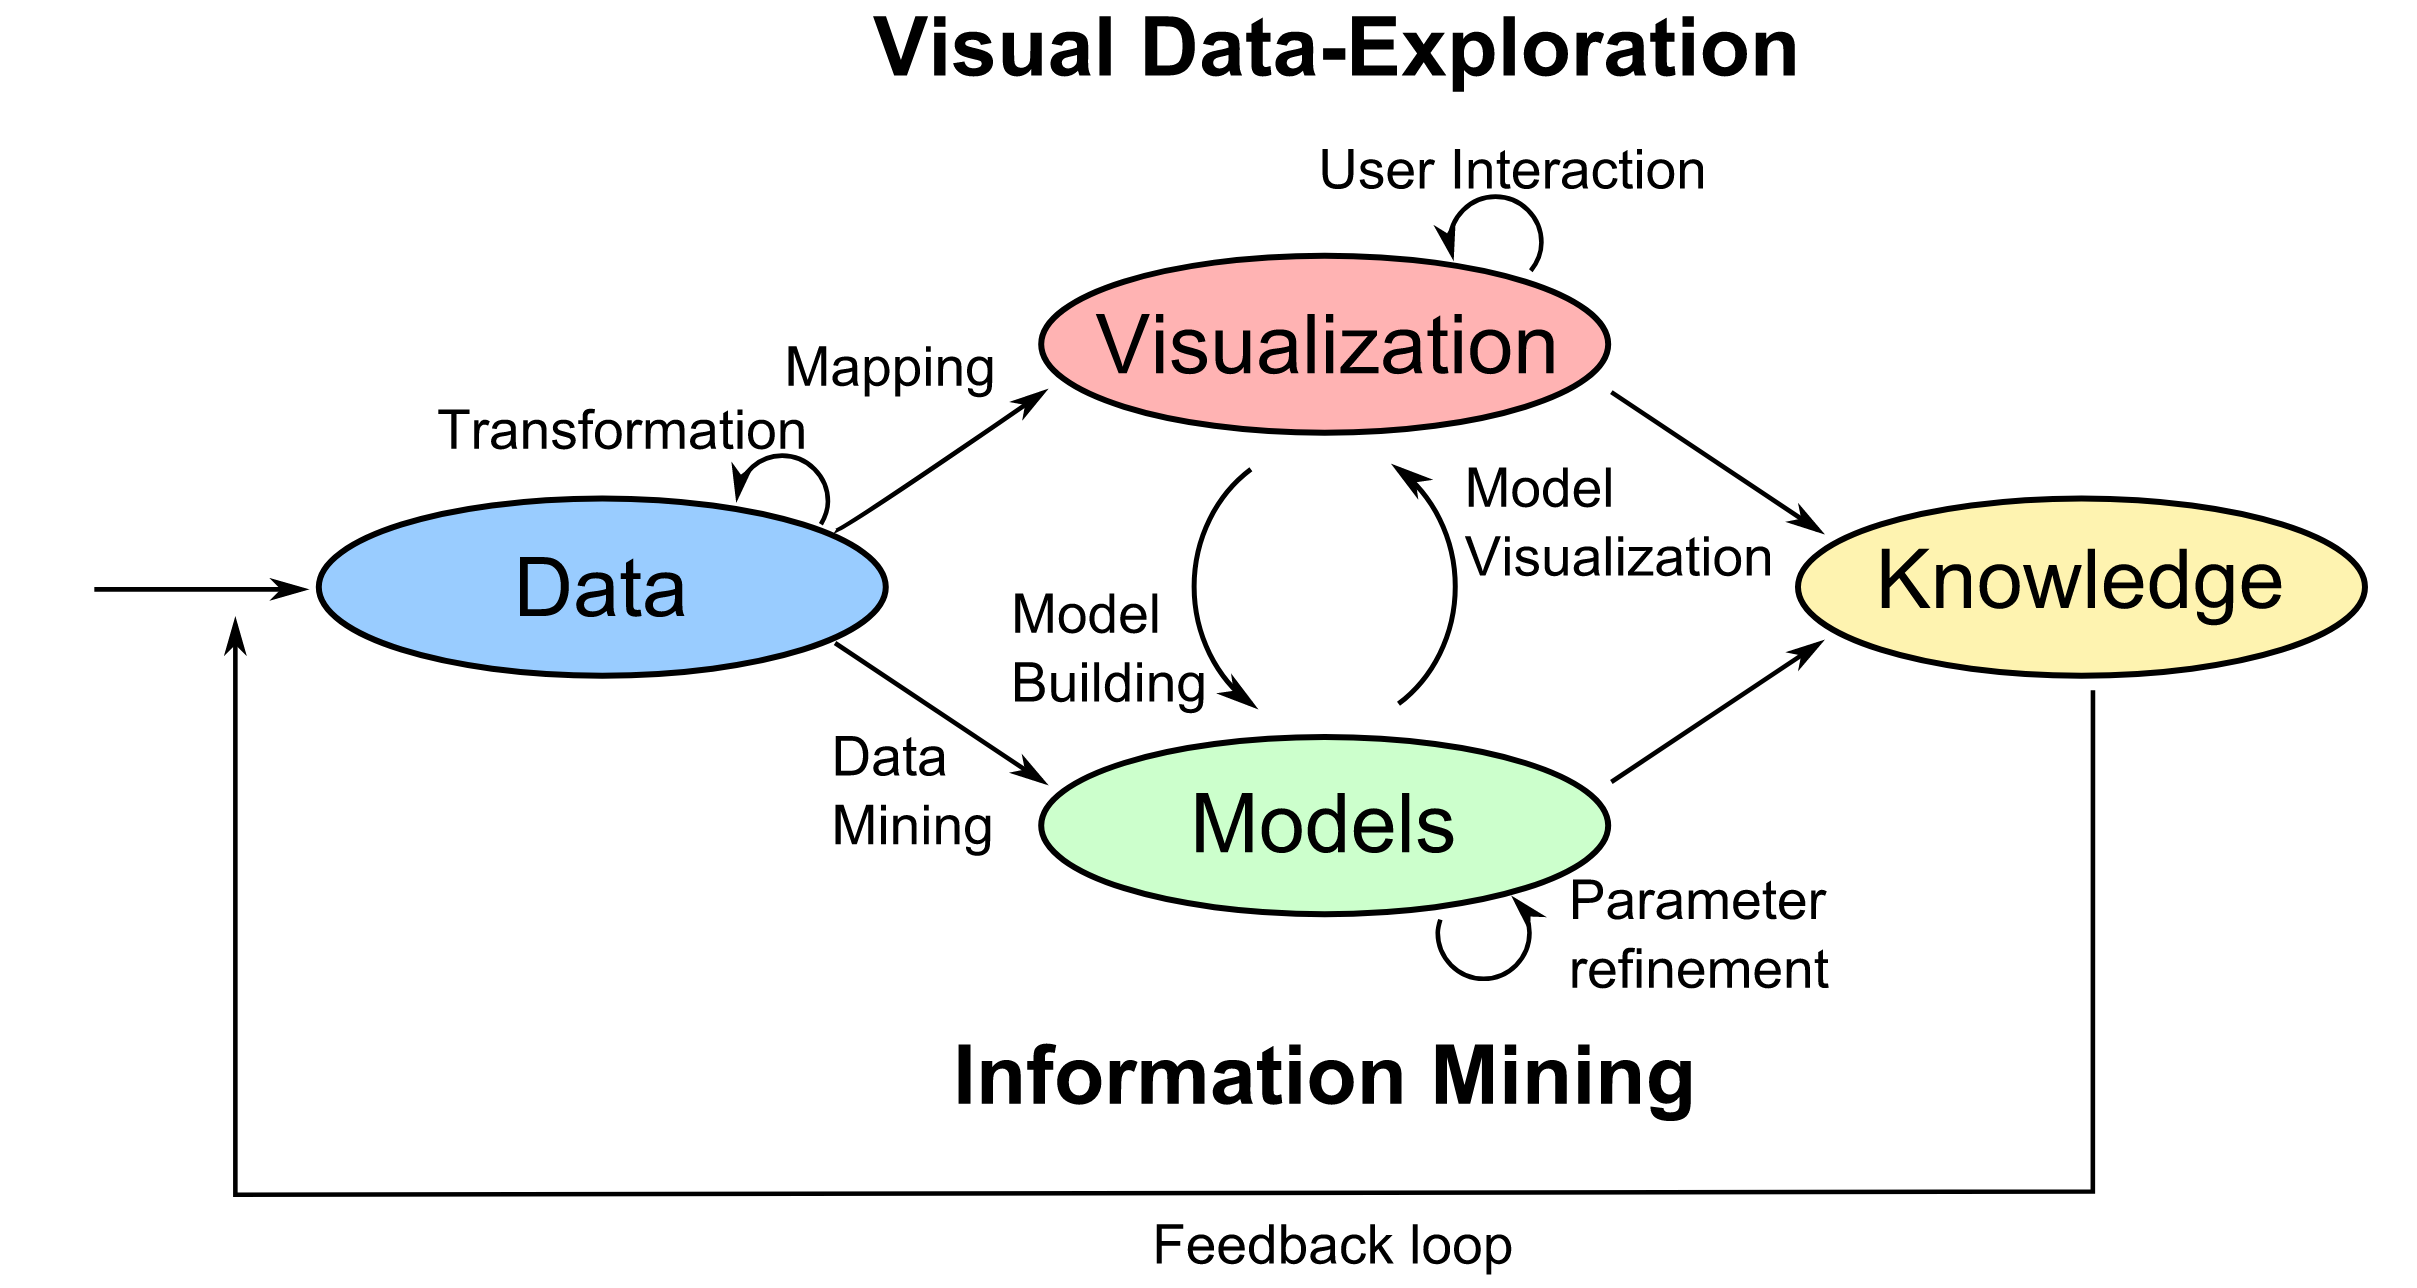
\includegraphics[width=1\textwidth]{static/figures/RelatedWork/Keim-VisualAnalytics.png}
    \caption{Abstraction of the VA process. It is characterized by continuous interactions between the data, visualizations, models, and knowledge. Image from \cite{keimVisualAnalyticsDefinition2008}.}
    \label{fig:keim-va}
\end{figure}
%Such interfaces aim at producing knowledge on the data, based on transformation of the data and interactions by the user.

\autoref{fig:keim-va} illustrate the schematic process of VA: the coupling of visualization and data mining models operated by the user through interaction lead to the generation of knowledge on the data.

If most widely used visual interface for \hsna do not yet provide complex interactions or data mining capabilities, more recent tools are oriented towards VA, as complex interactions and data mining capabilities can be a powerful support for social scientists to gain insight on the structure of their network, especially that the data they study keep growing in size and complexity \cite{kaplanVeniceTimeMachine2015}.


%EDA and VA are currently not widely used in HSNA, as social historians always have prior hypotheses before getting their data in shape.
%However, datasets that historians produce are getting bigger and bigger and VA tools are efficient in rapidly generating insights and new hypotheses.

%For example, clustering algorithms are often implemented in classical software for SNA such as Gephi and Pajek, allowing social scientists to explore potential interesting grouping of individuals in the network.

\section{Historical Social Networks Visual Analytics}\label{sec:intro-HSNV}

Most visual tools for SNA are designed for the analysis of already curated networks, without taking into account the context in which those networks have been produced, where they come from, and the workflow that led to their creation.
%Yet, social historians may need to generate several networks for their analsysis.
Currently, social historians spend a lot of time in their data acquisition, processing, and encoding steps which lead them to the construction of a network \cite{lemercierBackSourcesPracticing2021}.
They typically visualize and analyze their network at the end of this process, first to verify hypotheses they formulated during the inspection of their sources, then to gain a better view of the structure of the network, allowing them to potentially generate new hypotheses\cite{dufournaudCommentRendreVisible2018}.
%This can be explained in part because most VA tools focus only on this final analysis and not on the preprocessing steps.
%Social historians collect, annotate and clean their data using custom scripts and ad-hoc methods before doing any analysis.
However, research showed that all the steps preceding the analysis can introduce errors and misconceptions, especially since social scientists are often not trained in Computer Science and Data Science\cite{lemercier12FormalNetwork2015, alkadi2022}.
Social scientists usually visualize their network using SNA tools like Gephi\cite{Gephi}, Pajek\cite{pajek}, and NodeXl\cite{noauthor_nodexl_nodate} which encompass basic interactions, node-link visualization, SNA measure computations, and clustering algorithms.
Once they visualize their data, they typically notice errors and inconsistencies in the data, such as duplication of the same entities, merging of different entities, or geolocation errors \cite{alkadi2022}.
They, therefore, have to go back and forth between the visualization software and the encoding process which can be tedious, especially since it can be complicated to trace back the entities of the data model back to the original documents for correction.
VA tools which encompass the whole process of social historians should therefore be beneficial for the flow of their work and could help detect and correct errors or analysis plans way before the visualization of a finalised network.
VA could also help social scientist reflect on their network modeling process as historical documents can be modeled in various ways\cite{cristofoliAuxSourcesGrands2008}.
Yet, most visualization tools aimed at HSNA such as Gephi\cite{Gephi} or Pajek\cite{pajek} enforce simple network models, which visualization and analysis can often lead to trivial or distorted conclusions\cite{lemercier12FormalNetwork2015}.
Furthermore, the data mining capabilities proposed in those softwares are often based on black-box algorithms, which can be hard to interpret for social analysts.
For example, clustering algorithms are often included in such systems, letting social scientists partition networks into groups, but many algorithms exist in the literature, potentially giving diverse results.
Scientists often run several algorithms until finding a satisfying enough partition, which can bias the result of an analysis\footnote{We did not find any scientific production describing these potential issues when following such analyses. However, many social scientists refered to these problems to us in informal discussions.}.
Usability and traceability of the results are therefore primordial in VA interfaces aimed at supporting social historians in their analysis.

%Moreover, social scientists have been frustrated by current data mining tools as the results they get from tasks such as clustering and classification come from black-box algorithms and may mismatch their vision of the data.
%They thus often feel they do not have control over their analysis\cite{lepetitHistoireQuantitativeDeux1989}.
%One of the reasons is that automatic results can be hard to interpret, especially in disciplines such as History and Sociology, where users often have little knowledge of computer science.



\section{Contributions and Research Statement}\label{sec:contribution-and-research-statement}

The goal of this thesis is to characterize how \va can support social historians in their \hsna workflow.
Most \snv tools allow to visualize a finalised polished network and compute network measures, allowing historians to explore and answer sociological questions through network descriptions.
Howver, \va could propose more complex representations and interactions mechanisms, to go beyond simple visualization of networks.




As seen in \autoref{sec:intro-HSNV}, most \va tools for HSNA are focused on the final analysis of a polished network.
Furthermore, most widely used \snv interfaces let historians visualize their networks with node-link diagrams and compute network measures, which is often not necessary to answer complex historical questions.
\va could therefore 1) assist social historians in their overall workflow, starting at the documents' acquisition to the final analysis step, with the help of interaction and data mining mechanisms in the data acquisition, encoding, modeling steps, and 2) provide analysis mechanisms to answer complex historical questions from the network.
Instead of only providing analysis capabilities, we think VA could help social historians in their entire workflow, from data acquisition to analysis, instead of focusing only on the final steps.
%without losing the traceability to their original historical sources and the temporality of the phenomena they study.
The goal of this thesis is therefore to give answers to the high-level question ``How can VA support social historians in their entire HSNA process?''.
To answer this question, we first characterize the HSNA process from start to finish from discussions and collaborations with social historians, with the goal of identifying pitfalls that regularly arise and characterizing social historians' needs.
%From this, we give answers and directions to three questions that frequently arise in social scientists' workflows:
From this, we give answers and directions to three questions concerning the modeling aspect of \hsna and how \va and automatic tools can support social historians in different parts of their process:


\begin{description}
%    \item \textbf{Q1}: How should historians collect, annotate and model their historical documents, allowing them to answer their complex questions with HSNA methods?
%    \item \qone:  How to model relationships contained in historical documents into an analyzable network with the right balance between expressiveness and simplicity?
    \item \qone:  How to model relationships contained in historical documents into an analyzable network with the right balance between expressiveness and simplicity?
%    \item \qtwo:  What representations and interactions are efficient for social historians to answer complex historical questions and generate insight and hypotheses, while being easy enough to navigate?
    \item \qtwo:  What representations and interactions would allow social historians answer complex historical questions?
    \item \qthree: How to design VA tools and interactions that leverage algorithmic power but keep historians in control of their analysis and bias?
\end{description}


%Instead of only providing analysis capabilities, we think VA could help social historians in their entire workflow, from data acquisition to analysis, instead of focusing only on the final steps.
%Concerning the analysis step, VA tools should satisfy the constraints of social historians, i.e.\ being able to answer complex questions with effective visual representations, letting the user in control of the analysis loop and algorithmic results, and satisfying traceability to the original sources.
%%without losing the traceability to their original historical sources and the temporality of the phenomena they study.
%The goal of this thesis is therefore to give answers to the high-level question ``How can VA help social historians in their entire HSNA process?''.
%To answer this question, we first characterize the HSNA process from start to finish from discussions and collaborations with social historians, with the goal of identifying pitfalls and problems that regularly arise and characterizing social historians' needs.
%From this, we give answers and directions to three issues that frequently arise in social scientists' workflows:


%\begin{description}
%%    \item \textbf{Q1}: How should historians collect, annotate and model their historical documents, allowing them to answer their complex questions with HSNA methods?
%    \item \textbf{Q1}: How should historians model their documents into an analyzable network with the right balance between expressiveness and simplicity?
%    \item \textbf{Q2}: What representations and interactions are necessary for social historians to answer complex historical questions while being easy enough to navigate?
%    \item \textbf{Q3}: How to design VA tools and interactions that leverage algorithmic power but let historians in control of their analysis and without introducing bias?
%\end{description}

In \autoref{ch:hsna-process-and-network-modeling}, we start by describing the HSNA workflow and identify recurring pitfalls we encountered in our collaborations with historians and answer \qone by proposing a network model for mdeling historical documents..
In the following \autoref{ch:combinet}, we give answers to \qtwo by providing a \va interface to explore \modelplural, with queries and comparison interactions with the aim of letting historians detect inconsistencies, answer their questions, and generate interesting hypotheses.
Finally, in \autoref{ch:pk-clustering}, we propose PK-Clustering, a mixed-initiative clustering technique for social scientists based on their prior knowledge, algorithmic consensus, and traceability of results, as a concrete example of a system providing answers to \qthree.


%This thesis is centered around two research questions: first, the proposition of an efficient network model to represent historical sources and follow HSNA, with associated visualizations to show and explore this type of network. Secondly, elaborating visual analytics tools specifically designed for this type of data, with the right balance between algorithmic power, simplicity and interpretability for the social scientists, who need to be in control of the analysis. We first [tell plan]


%Observations:
%\begin{description}
%    \item \textbf{O1}: Social scientists have trouble processing and modeling their historical documents into a clean, consistent and analyzable network. The process is not easy and straightforward and more resources should give insight on how to do it correclty.
%    \item \textbf{O2}: SNA have been criticized for giving trivial results and visual analysis tools used only for producing good-looking pictures.
%    \item \textbf{O3}: Historians have been frustrated with automatic tools and algorirthms to analyze their data, as they have a strong knowledge of their subject and not everything is modeled inside the network, and current tools do not allow them to express this knowledge.
%\end{description}
%
%Research Questions
%\begin{description}
%    \item \textbf{Q1}: How should historians collect, annotate and model their historical documents, allowing them to answer their complex questions with HSNA methods?
%    \item \textbf{Q2}: What representations and interactions are necessary for social historians to answer question, potentially complex?
%    \item \textbf{Q3}: How to design tools and interactions that let historians in control of the analysis loop, without introducing bias?
%\end{description}





%\section{Network models and representations}
%
%Person-to-person simple node-link diagram is still the most widely used network representation is SNA, and most SVA tools only include this type of representation.
%This visualization shows the persons as nodes, and social ties as links and displays them in a way to minimize the number of crossings to increase the readability.
%However, historians very often have access to richer and more diverse information through the historical documents they study.
%The documents can refer to coexistent complex social relationships which link several people together with different roles.
%These cannot be modeled with simple person-to-person links, without losing some information on the social implication of these relationships.
%Moreover, documents often give access to other information related to the event they refer to, such as the time, the location or the roles of the different persons mentioned.
%For example, marriage acts often indicate the date and the place of the event, and mention persons under different roles : the spouses, the witness, the parents, the priest etc.
%Additional information related to persons can also be mentioned, such as their age, origin or profession.
%It is clear that simply using a person network model won’t encapsulate the whole complexity of the data and will simplify the social relationship. This is a common issue in SNA and HSNA [REF Lemercier] and more complex network models are needed. However, complexity
%along with visual analysis tools to explore them.
%
%\section{Usability Issues}
%
%One of the aims of Visual Analytics is to provide automatic or semi-automatic processing and analysis tools with data mining and machine learning algorithms, to help end users make sense of their data and find interesting patterns and relationships.
%However, current social network visual analytics systems are still very algorithm oriented, and do not provide many controls to historians and sociologists who usually feel off the analysis loop when the system provides automatic and algorithmic results. One of the reason is because automatic results can be hard to interpret, especially in a discipline such as History or Sociology, where users often have little knowledge on computer science.
%One example is the automatic detection of community structures using network clustering algorithms. Social networks are known to have a community-like structure, meaning that the probability of a link existing between two random person nodes is not uniform, and that people tend to agglomerate in groups, who have more social ties between them than with other persons in the network.
%There are a lot of existing clustering algorithms which aim to automatically find these groups, by optimizing measures such as the modularity or using propagation models.
%However, clustering is an ill-defined problem, and several good partitions may coexist for the same network, and which can have several interpretations in a SNA. Most SNA/SVA tools such as Gephi or NodeXl provide several well-known clustering algorithms such as Girvan-Newman, Louvain or Clauset-Newman-Moore, but do not provide much guidance on how to use them and interpret their results.
%Social Scientists often try several ones in the list of algorithms proposed until finding a convenient result, in the eyes of the analysis they want to follow.
%This leads to a non-satisfactory analysis process, as historians are out of the loop and have few decisions on the results. This usability issue is the same for automatic processes with no universal ground truth.
%
%\section{Contribution and research statement}
%
%This thesis is centered around two research questions: first, the proposition of an efficient network model to represent historical sources and follow HSNA, with associated visualizations to show and explore this type of network. Secondly, elaborating visual analytics tools specifically designed for this type of data, with the right balance between algorithmic power, simplicity and interpretability for the social scientists, who need to be in control of the analysis. We first [tell plan]
%
%
%Observations:
%\begin{description}
%    \item \textbf{O1}: Social scientists have trouble processing and modeling their historical documents into a clean, consistent and analyzable network. The process is not easy and straightforward and more resources should give insight on how to do it correclty.
%    \item \textbf{O2}: SNA have been criticized for giving trivial results and visual analysis tools used only for producing good-looking pictures.
%    \item \textbf{O3}: Historians have been frustrated with automatic tools and algorirthms to analyze their data, as they have a strong knowledge of their subject and not everything is modeled inside the network, and current tools do not allow them to express this knowledge.
%\end{description}
%
%Research Questions
%\begin{description}
%    \item \textbf{Q1}: How should historians collect, annotate and model their historical documents, allowing them to answer their complex questions with HSNA methods?
%    \item \textbf{Q2}: What representations and interactions are necessary for social historians to answer question, potentially complex?
%    \item \textbf{Q3}: How to design tools and interactions that let historians in control of the analysis loop, without introducing bias?
%\end{description}